\documentclass[11pt,letterpaper]{article}
\usepackage[margin=0.90in,headheight=15pt,footskip=25pt]{geometry}
\usepackage[T1]{fontenc}
\usepackage{libertinus}
\usepackage{microtype}
\usepackage{amsmath,amssymb,amsthm,mathtools}
\usepackage{booktabs,tabularx,array,multirow,enumitem}
\usepackage{tikz}
\usetikzlibrary{arrows.meta,positioning,calc,fit,shapes.geometric}
\usepackage{fancyhdr,lastpage,needspace}
\usepackage{xurl}
\usepackage[hidelinks]{hyperref}
\usepackage[nameinlink,noabbrev]{cleveref}
\usepackage{titlesec}
\usepackage{xcolor}
\definecolor{ink}{RGB}{25,25,25}
\definecolor{mute}{RGB}{86,86,86}
\definecolor{papergray}{RGB}{244,244,244}
\definecolor{linegray}{RGB}{145,145,145}
\hypersetup{pdftitle={Symphonies of Automated Theorem Provers: Cooperative Dream Histories, Certified Gestalt, and the Limits of Federated Advantage},pdfauthor={Brian Tenneson; AI-assisted exposition},pdfsubject={Cooperative proof search, ATP dreaming, MUSIC and SYMPHONY, proof certificates},pdfkeywords={automated theorem proving, AMLD+0, dream histories, distributed theorem proving, gestalt, symphony, evidence, proof verification}}
\color{ink}
\setlength{\parindent}{1.25em}
\setlength{\parskip}{0.09em}
\setlength{\emergencystretch}{2em}
\linespread{1.018}
\setlist[itemize]{topsep=4pt,itemsep=2pt,leftmargin=1.6em}
\setlist[enumerate]{topsep=4pt,itemsep=3pt,leftmargin=1.8em}
\titleformat{\section}{\Large\bfseries}{\thesection.}{.6em}{}
\titleformat{\subsection}{\large\bfseries}{\thesubsection.}{.6em}{}
\titlespacing*{\section}{0pt}{13pt}{6pt}
\titlespacing*{\subsection}{0pt}{10pt}{4pt}
\pagestyle{fancy}
\fancyhf{}
\fancyhead[L]{\small\textsc{Symphonies of Automated Theorem Provers}}
\fancyhead[R]{\small\textsc{Research exposition / 2026}}
\fancyfoot[C]{\small\thepage\ / \pageref{LastPage}}
\renewcommand{\headrulewidth}{0.3pt}
\newtheorem{theorem}{Theorem}[section]
\newtheorem{lemma}[theorem]{Lemma}
\newtheorem{proposition}[theorem]{Proposition}
\newtheorem{corollary}[theorem]{Corollary}
\theoremstyle{definition}
\newtheorem{definition}[theorem]{Definition}
\newtheorem{example}[theorem]{Example}
\newtheorem{question}[theorem]{Research question}
\theoremstyle{remark}
\newtheorem{remark}[theorem]{Remark}
\newcommand{\PSet}{\mathcal{P}}
\newcommand{\Fin}{\operatorname{Fin}}
\newcommand{\Cn}{\operatorname{Cn}}
\newcommand{\Runs}{\operatorname{Runs}}
\newcommand{\Dream}{\mathcal{D}}
\newcommand{\Music}{\operatorname{MUSIC}}
\newcommand{\Sym}{\operatorname{SYMPHONY}}
\newcommand{\Bank}{\operatorname{BANK}}
\newcommand{\Board}{\operatorname{Board}}
\newcommand{\Sound}{\operatorname{Sound}}
\newcommand{\Cert}{\operatorname{Cert}}
\newcommand{\Acc}{\operatorname{Accept}}
\newcommand{\Proj}{\operatorname{Proj}}
\newcommand{\Span}{\operatorname{Span}}
\newcommand{\defeq}{\mathrel{\mathop:}=}
\newcommand{\mref}[1]{\textnormal{[\ref{#1}]}}
\begin{document}
\begin{center}
{\LARGE\bfseries Symphonies of Automated Theorem Provers\par}
\vspace{4pt}
{\large\itshape Cooperative Dream Histories, Certified Gestalt, and the Limits of Federated Advantage\par}
\vspace{9pt}
{\large Brian Tenneson\par}
\vspace{3pt}
{\small Research conception; AI-assisted expository development\par}
\vspace{4pt}
{\small November 3, 2026 \quad $\cdot$ \quad Research article, version 2.0\par}
\end{center}
\vspace{2pt}
\begin{center}
\begin{minipage}{.94\textwidth}
\footnotesize\noindent\textbf{AI authorship and reliability notice.} This article contains human-originated research concepts developed with AI-assisted mathematical exposition. The complete statement of authorship, scope, and verification limitations appears as the final page, after the references and glossary.
\end{minipage}
\end{center}
\vspace{7pt}
\begin{abstract}
Can five cooperating automated theorem provers (ATPs) produce a checkable proof unavailable to any one member under its initial evidence restrictions? We model an ATP symphony as a family of legal execution scores recording local dreams, causal order, authenticated messages, and verification events. Each dream is a union of typed reports; an ATP's MUSIC is the powerset of its possible dreams. We distinguish the whole score family from the subfamily witnessing an accepted target proof. A five-member Horn instance yields a coalition-minimal target, and an explicit finite generalized-board-game protocol constructs a legal certificate-bearing run. We show when a score preserves proof-relevant history and prove that verifier-gated admissions conserve the global logical consequence set. Counterexamples explain why unordered reports lose information and why individually possible dreams may be incompatible. Conditional simulation and cost-accounting results rule out unconditional claims of speedup. The Horn witness and related federation results have precedents in Tenneson's earlier dreaming paper; the structured score and its fidelity conditions are developed here as an extension. The results concern stipulated mathematical models, not an implemented AMLD+0 federation, independently machine-checked proofs, or measured computational improvements.
\end{abstract}
\noindent\textbf{Keywords:} automated theorem proving; cooperative proof discovery; dreaming; generalized board game; MUSIC; SYMPHONY; coalition-minimal proofs; certificates; AMLD+0; resource accounting.
\tableofcontents
\vspace{4pt}

\section{The motivating question and the scope of the answer}
In ordinary theorem proving, a formal claim is established by a derivation from declared premises using accepted rules. A proof-search program can discover candidate derivations by enumeration, heuristic guidance, learned predictions, or external advice. None of these search mechanisms should be confused with the rule that makes a derivation acceptable: an independently defined checking procedure.

Now consider five ATPs that can inspect different evidence, dream about earlier computations, and exchange claims through authorized channels. There are three distinct questions. First, can the joint evidence entail a target that no participant's evidence entails? Second, can that target be discovered through an actual legal cooperative dreaming run? Third, does an explicitly musical or score-like representation of that run preserve what is needed to check the final proof and provide any additional computational benefit? The answers are, respectively: \emph{yes by an elementary construction}; \emph{yes under a specified operational model}; and \emph{soundness can be preserved, while improved cost requires separate assumptions and experiments}.

The first two answers are not presented as new priorities. In Tenneson's \emph{Dreaming in a Five-ATP Federation}, Definition 6.1 and Theorem 6.2 formulate and prove a five-member Gestalt witness, Theorem 7.1 builds a legal five-member dreaming model with certified deposits, and Theorems 4.1--4.2 address conservativity \cite{tenneson-dreaming}. The purpose here is to supply all definitions and proofs needed to understand those ideas without consulting the earlier paper, then ask what the proposed word \emph{symphony} adds. The methodological distinction between invariant proof standards and variable search geometry is also prominent in \emph{The Invariant Core and the Geometry of Settlement} \cite{tenneson-core}.

\paragraph{Claim categories.} A \emph{definition} introduces vocabulary; an \emph{internal theorem} is established from explicit assumptions in this paper; a \emph{source precedent} attributes an antecedent result; a \emph{design claim} specifies an intended interface; and an \emph{empirical claim} requires an experiment or measured system. Keeping these separate is necessary for a meaningful proof-theoretic interpretation of musical structure.

\section{The underlying mathematical machine}
\subsection{A formal language, evidence, and proof checking}
Fix a propositional language $\mathcal L$ with a sound derivation relation $\vdash$ and semantic consequence $\models$. For the central example, ordinary classical propositional logic is sufficient. Let $\Gamma\subseteq\mathcal L$ be a fixed common background theory; let $E_i\subseteq\mathcal L$ be the initially available evidence of ATP $A_i$, where $i\in\{1,\dots,5\}$. The \emph{globally authorized object-level premise base}, whose members are permitted assumptions rather than automatically established truths, is
\begin{equation}\label{eq:base}
\Sigma_0\defeq\Gamma\cup\bigcup_{i=1}^5 E_i.
\end{equation}
The consequence operator is $\Cn(X)\defeq\{\varphi:X\vdash\varphi\}$; the soundness contract requires $X\vdash\varphi\implies X\models\varphi$. We use an ordinary monotone, idempotent classical deductive closure. In the witness below, authenticated member packets authorize use of $a_i$ \emph{as premises} in $\Sigma_0$; authentication is not a proof that each $a_i$ is unconditionally true. A checker $V$ takes a context, a proposed conclusion, and a proof artifact, and accepts only if the declared calculus and dependencies validate the artifact. We assume that $V$ is sound relative to the specified formal calculus; this is a mathematical assumption, not a claim that a particular piece of software has been audited.

\begin{definition}[Certified BANK and speculative Board]
The \emph{BANK} contains accepted typed records, each identifying the exact statement, context, proof or evidence payload, dependency chain, producing member, time, verification rule/version, and authorization status. The \emph{Board} contains tentative hypotheses, search plans, unverified proof fragments, and proposed exchanges. A Board entry has no theorem-admission power. A verifier-gated deposit is permitted only after all proof obligations and foreign assumptions are discharged or explicitly retained in a conditional sequent.
\end{definition}

An ATP may also possess a historical or awareness BANK, containing verified statements \emph{about} prior computational events. Those records are not automatically new object-level axioms. For example, the proposition that a player previously read a lemma is different from a derivation of the lemma.

\subsection{Five hosts, internal dream players, and Player Zero}
Let $\mathcal F=(A_1,A_2,A_3,A_4,A_5,\Omega,V,\Sigma_0)$ be one federation. Each $A_i$ hosts $r_i\ge2$ internal game processes $P_{i,1},\ldots,P_{i,r_i}$; these may include processes called \emph{Knowledge}, \emph{Awareness}, and \emph{Intuition}. The exact count of internal processes is design-dependent. Thus \emph{five ATP hosts} does not mean five internal faculties. A local board-player $P_{i,0}$ may authorize internal moves without being a sixth ATP.

A separate coordinator, called \emph{Player Zero} or $\Omega$, may schedule members, route admissible messages, and allocate resource budgets. It cannot declare a conjecture proved by fiat. In an AMLD+0 settlement profile, the five \emph{investigative roles} are proof ($P$), refutation ($R$), dependence ($D$), independence ($I$), and consistency ($C$); the report $U$ means no accepted terminal result. These role labels are contracts and need not coincide one-to-one with the five ATP hosts. The protocol is described in \cite{tenneson-wcf,tenneson-bootstrap}.

\subsection{An infinite but locally finite generalized board}
A convenient generalized board is the four-neighbor grid $G=(\mathbb Z^2,\sim)$, where $(x,y)\sim(x',y')$ when $|x-x'|+|y-y'|=1$. Its vertices are infinite, but every vertex has exactly four neighbors. A complete machine state contains more than visible piece positions: it includes the relevant game rules, permitted actions, evidence handles, BANK-copy state, message queues, and schedule. \emph{Local finiteness} of the grid by itself does not imply that the state graph is finitely branching; the legal-action rule must also constrain each state's enabled moves when finite branching is needed.

\begin{definition}[Legal federated run]
A run from checkpoint $c$ is a finite or infinite sequence
\[
\rho=(X_0\xrightarrow{e_1}X_1\xrightarrow{e_2}\cdots),\qquad X_0=c,
\]
where each transition $e_j$ is permitted by the complete state, the local rule and the federation authorization policy. Each transition records the acting host and player, any evidence-bearing action, authenticated message, verifier decision, and charged cost. The collection of finite legal runs from $c$ is $\Runs(\mathcal F,c)$. We require a set-sized state universe and a set-sized event alphabet with a formal transition predicate; finite runs then form a set. This prevents an implicit appeal to a collection of all histories across proper-class state spaces.
\end{definition}

\begin{definition}[Dream]
An ATP \emph{dreaming episode} is a nonempty legal segment in which a member conducts an evidence-dependent read, reconstruction, hypothetical search, duplicate check, or candidate verification from an authorized record; idle turns alone do not qualify. An ordinary \emph{location report} is a set of atomic board or event facts. The dream's report content is the union
\begin{equation}\label{eq:dream}
 d(h)\defeq\bigcup_{r\in\mathcal R(h)}r,
\end{equation}
where $\mathcal R(h)$ is the collection of reports emitted during episode $h$. A \emph{cross-member dream} additionally uses a received authorized evidence packet. Unless reports carry time/order tags, $d(h)$ is not the complete history $h$.
\end{definition}

\begin{figure}[htbp]
\centering
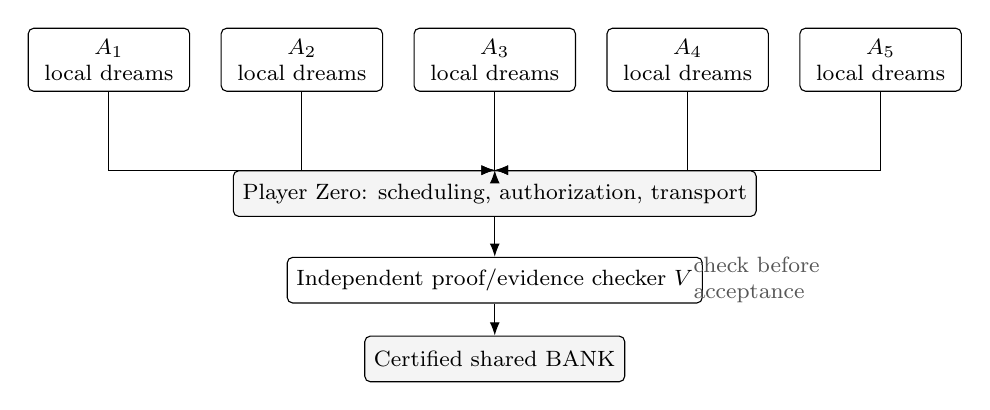
\begin{tikzpicture}[>=Latex, font=\footnotesize, box/.style={draw,rounded corners=2pt,minimum width=2.05cm,minimum height=.8cm,align=center},smallbox/.style={draw,rounded corners=2pt,minimum width=2.05cm,minimum height=.58cm,align=center}]
\node[box] (a1) at (0,1.7) {$A_1$\\local dreams};
\node[box] (a2) at (2.45,1.7) {$A_2$\\local dreams};
\node[box] (a3) at (4.9,1.7) {$A_3$\\local dreams};
\node[box] (a4) at (7.35,1.7) {$A_4$\\local dreams};
\node[box] (a5) at (9.8,1.7) {$A_5$\\local dreams};
\node[smallbox,fill=papergray,minimum width=5.1cm] (coord) at (4.9,.0) {Player Zero: scheduling, authorization, transport};
\node[smallbox,minimum width=4.3cm] (gate) at (4.9,-1.1) {Independent proof/evidence checker $V$};
\node[smallbox,minimum width=3.2cm,fill=papergray] (bank) at (4.9,-2.1) {Certified shared BANK};
\foreach \i in {1,...,5} {\draw[->] (a\i.south) -- (coord.north -| a\i.south) -- (coord.north);}
\draw[->] (coord) -- (gate);
\draw[->] (gate) -- (bank);
\node[align=left,anchor=west,text=mute] at (7.3,-1.1) {check before\\acceptance};
\end{tikzpicture}
\caption{A five-host cooperative dreaming architecture. Arrows indicate admissible proposal and evidence flows, not automatic logical entailment. Player Zero controls routing but not truth.}
\label{fig:architecture}
\end{figure}

\section{From individual MUSIC to cooperative SYMPHONY}
\subsection{The literal MUSIC construction}
Fix a host $A_i$, a certified local BANK $B_i$, internal player set $P_i$, and complete starting or intermediate condition $c_i$. Let $\Dream_i(c_i)$ be the set of distinct report-union dreams obtainable through legal finite episodes under those conditions. Assume a set-sized reporting universe $U_i$, with every dream a subset of $U_i$ and legal report-union membership defined by a predicate with set parameters. Thus $\Dream_i(c_i)\subseteq\PSet(U_i)$ exists by Separation; the previously stipulated set-sized finite-run space is an alternative sufficient construction.

\begin{definition}[Potential MUSIC]
The \emph{MUSIC} of host $A_i$ relative to its frozen conditions is
\begin{equation}\label{eq:music}
\boxed{\Music(A_i,B_i,P_i,c_i)\defeq\PSet(\Dream_i(c_i)).}
\end{equation}
It is the set of \emph{all subsets of possible dreams}, not one sound file, one melody, or necessarily a family that can be performed together.
\end{definition}

\begin{proposition}[Recovery and cardinality]
For any set $D$ of possible dreams, $D=\bigcup\PSet(D)$. If $|D|=m<\infty$, then $|\PSet(D)|=2^m$; if $D$ is infinite, $|\PSet(D)|>|D|$.
\end{proposition}
\begin{proof}
Each $d\in D$ appears in the singleton subset $\{d\}\in\PSet(D)$, while every element of every member of $\PSet(D)$ belongs to $D$. Thus the union recovers $D$. The cardinality statements are the standard finite subset count and Cantor's theorem.
\end{proof}

This theorem is elementary set theory. Its importance is conceptual: MUSIC specifies \emph{potential} dream collections, not a record of which collections have appeared during one joint execution.

\subsection{What is jointly realizable?}
\begin{definition}[Local realization complex]
Let $\operatorname{Dreams}(\rho)$ denote all report-union dreams actually produced during one finite legal run $\rho$. Define
\begin{equation}\label{eq:localcomplex}
K_i(c_i)\defeq\{X\in\Fin(\Dream_i(c_i)):\exists\rho\text{ legal from }c_i,\ X\subseteq\operatorname{Dreams}(\rho)\}.
\end{equation}
Here $\Fin(D)$ is the collection of finite subsets of $D$. This is \emph{jointly realizable MUSIC} in the finitary sense.
\end{definition}

\begin{proposition}[Downward closure]
Assume at least one finite legal run exists. If $X\in K_i(c_i)$, every $Y\subseteq X$ also belongs to $K_i(c_i)$; in particular $\varnothing\in K_i(c_i)$. Consequently $K_i(c_i)$ is an abstract simplicial complex on the set of dreams appearing in some finite run. To take all of $\Dream_i(c_i)$ as its vertex set, also require realization coverage.
\end{proposition}
\begin{proof}
Choose a run witnessing $X\subseteq\operatorname{Dreams}(\rho)$. Then $Y\subseteq X\subseteq\operatorname{Dreams}(\rho)$, so the same run witnesses $Y$. The empty set is included because the run family is nonempty. A dream not realized in any such run need not be a vertex.
\end{proof}

The qualification matters: a pair of individually possible dreams may conflict over a consumable token, a fixed deadline, or mutually exclusive authorization. The powerset $\PSet(\Dream_i)$ includes the pair, but $K_i$ need not. Combinatorial topology appears here because \emph{compatibility of finite dream sets} is downward closed, not because music necessarily creates a new topological theorem.

\subsection{A score is a structured execution, not an unordered bag}
Fix a legal finite federation run $\rho$. Its \emph{local projection} $\pi_i(\rho)$ is the ordered sequence of events, reports, costs, and dream boundaries attributable to $A_i$. Let $H_\rho$ be the relevant intermember \emph{happens-before} relation: local event order, authenticated send-before-receive edges, and their transitive closure. Let $Q_\rho$ be the typed evidence-transfer and checker-response ledger. Let $G_\rho$ be an ordered global-event ledger containing coordinator operations, checker steps, costs, state changes and any other transition-relevant events not wholly captured by host projections. All records are relative to the checkpoint $c$. A full replay of a run requires that these components jointly retain all state-affecting transitions; a lossy logging scheme may still be useful for a narrower purpose.

\begin{definition}[Federation score and SYMPHONY]
A \emph{federation score} is an encoded tuple
\begin{equation}\label{eq:score}
S(\rho)\defeq E\bigl(\pi_1(\rho),\ldots,\pi_5(\rho),H_\rho,Q_\rho,G_\rho\bigr),
\end{equation}
where $E$ is a declared encoding into a space of structured scores. The \emph{SYMPHONY} of federation $\mathcal F$ from checkpoint $c$ is
\begin{equation}\label{eq:sym}
\boxed{\Sym(\mathcal F,c)\defeq\{S(\rho):\rho\in\Runs(\mathcal F,c)\}.}
\end{equation}
For target $g$, let $\operatorname{cert}_g(\rho)=1$ mean that a packet proving $g$ under the frozen, authorized premises has been independently checked and accepted in $\rho$ (and $0$ otherwise). Define the \emph{certified-performance subfamily} by
\[
\Sym^{\mathrm{cert}}_g(\mathcal F,c)\defeq
\bigl\{S(\rho):\rho\in\Runs(\mathcal F,c),\ \operatorname{cert}_g(\rho)=1\bigr\}.
\]
For a lossy $E$, the same score may have both successful and unsuccessful witnessing runs; membership in this existentially defined subfamily need not be recognizable from the score alone. Certificate faithfulness plus rechecking of its recovered packet supplies the necessary operational distinction. A \emph{certified movement} is a score $S(\rho_{\le t})$ of a finite legal run prefix containing such an acceptance, from which the accepted proof can be rechecked. It is a literal prefix of $S(\rho)$ only if the chosen encoding preserves prefixes; this is not required of arbitrary $E$. An \emph{audible rendering} is an optional map from a score to musical notes, rhythms and timbres; sound generation is not a prerequisite of the definition.
\end{definition}

The full set $\Sym(\mathcal F,c)$ includes uncertified or even dream-free legal runs; an arbitrary score is not automatically a proof. The encoding $E$ must not be assumed injective without evidence. For example, an interpretation that maps all moves of a player to a repeated note may be musically coherent but mathematically lossy. Conversely, serialization followed by a one-to-one code of bytes as note events yields a score that is lossless, albeit not necessarily aesthetically meaningful. The semantic conditions for a \emph{useful} score are established below.

\begin{figure}[htbp]
\centering
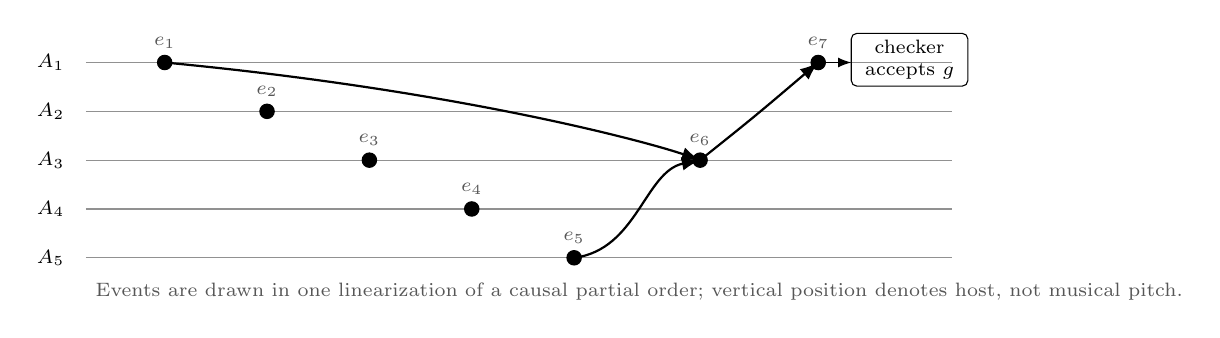
\begin{tikzpicture}[>=Latex,font=\scriptsize]
\foreach \y/\name in {0/$A_5$, .62/$A_4$, 1.24/$A_3$, 1.86/$A_2$, 2.48/$A_1$} {
  \node[anchor=east] at (-.15,\y) {\name};
  \draw[linegray] (0,\y) -- (11,\y);
}
\foreach \x/\y/\t in {1/2.48/1, 2.3/1.86/2, 3.6/1.24/3, 4.9/.62/4, 6.2/0/5, 7.8/1.24/6, 9.3/2.48/7} {
  \filldraw[black] (\x,\y) circle (2.6pt);
  \node[anchor=south,text=mute] at (\x,\y+.06) {$e_{\t}$};
}
\draw[->,line width=.8pt] (1,2.48) .. controls (4.8,2.12) and (7.2,1.45) .. (7.8,1.24);
\draw[->,line width=.8pt] (6.2,0) .. controls (7,.1) and (7.1,1.1) .. (7.8,1.24);
\draw[->,line width=.8pt] (7.8,1.24) .. controls (8.5,1.8) .. (9.3,2.48);
\draw[rounded corners=2pt] (9.72,2.18) rectangle (11.2,2.85);
\node[align=center] at (10.46,2.52) {checker\\accepts $g$};
\draw[->] (9.3,2.48) -- (9.72,2.48);
\node[anchor=west,text=mute] at (0,-.43) {Events are drawn in one linearization of a causal partial order; vertical position denotes host, not musical pitch.};
\end{tikzpicture}
\caption{Schematic symphonic score with five local voices. Local order and cross-host dependencies make it more informative than a union of untagged location reports.}
\label{fig:score}
\end{figure}

\section{Preservation: what a symphony must remember}
\subsection{A counterexample to naive union encoding}
\begin{example}[Same set, different histories]\label{ex:loss}
Take legal paths $h_1=(x,y,z)$ and $h_2=(x,y,x,y,z)$. If each report contains only its visited site, both dream unions equal $\{x,y,z\}$. Yet $h_2$ has two additional steps, potentially higher charged cost, and additional opportunities for reads or verifier actions. Therefore the map $h\mapsto\bigcup\mathcal R(h)$ is not generally injective and cannot by itself preserve all operational or verification facts.
\end{example}

A repair is to use unique event records, such as $(\text{host},\text{player},\text{epoch},\text{site},\text{payload},\text{evidence ID})$, including a causal predecessor relation when necessary. Their union retains individual identity; a score still needs an explicit reconstruction rule for order and dependencies. A distinct remedy is to retain the original trace separately and use the musical union only as an index.

\begin{definition}[Certificate-faithful score]
Let $W(\rho)$ denote the exact sequence of accepted, rejected, or pending verification packets and the scoped premises on which each verdict depends. A score encoding is \emph{certificate-faithful} for a class of runs $\mathcal R$ when a decoder $D_W$ satisfies
\[
D_W(S(\rho))=W(\rho)\qquad(\rho\in\mathcal R),
\]
up to an explicitly declared, verifier-valid equivalence of certificate artifacts. A stronger \emph{replay-faithful} score permits reconstruction of the checkpoint-relative ordered transition sequence, including all transition-relevant events, messages, and costs. Certificate faithfulness does not require the entire run to be recoverable.
\end{definition}

\begin{proposition}[Factorization criterion for sufficient information]\label{prop:factor}
Let $S:H\to\mathcal S$ be any representation of histories and $f:H\to Y$ any history-dependent property or artifact. There exists $\widehat f:\operatorname{im}(S)\to Y$ with $f=\widehat f\circ S$ if and only if
\[
S(h)=S(h')\Longrightarrow f(h)=f(h')\qquad\text{for all }h,h'\in H.
\]
\end{proposition}
\begin{proof}
If $f=\widehat f\circ S$, equal scores produce equal values. Conversely define $\widehat f(s)=f(h)$ for any $h$ such that $S(h)=s$. The hypothesis makes this definition independent of the choice of $h$.
\end{proof}

Applying \cref{prop:factor} with $f=W$ gives an exact criterion for when a score preserves verifier-relevant evidence; applying it with $f=\text{cost}$ tests preservation of charges. This criterion is new exposition of a standard factorization fact. It aligns with the stronger bidirectional quotient conditions of Proposition 11.2 in \cite{tenneson-dreaming}, which preserve enabled actions, admitted evidence views, checker decisions, novelty, and exact transition costs.

\subsection{A soundness theorem}
\begin{theorem}[Verifier-gated conservativity of symphonic search]\label{thm:sound}
Assume: (i) a frozen shared base $\Sigma_0$, with every initial accepted object-level BANK claim already in $\Cn(\Sigma_0)$; (ii) each later proposed BANK addition is independently verified as a derivation from $\Sigma_0$ and previously certified consequences, with all imported assumptions and theory translations checked; and (iii) MUSIC or SYMPHONY may alter proposal order, scheduling, or candidate selection but cannot bypass the checker. Then at every finite event horizon $t$,
\begin{equation}\label{eq:conservation}
B_t\subseteq\Cn(\Sigma_0),\qquad
\Cn(\Sigma_0\cup B_t)=\Cn(\Sigma_0),
\end{equation}
where $B_t$ denotes the accepted object-level formulas not already in $\Sigma_0$.
\end{theorem}
\begin{proof}
Proceed by induction on accepted deposits. Initially $B_0\subseteq\Cn(\Sigma_0)$ by the seed condition. If a new formula $\varphi$ is accepted, its verifier-approved derivation uses only $\Sigma_0$ and previously accepted formulas under sound, scope-preserving rules. By the induction hypothesis all imported predecessor formulas follow from $\Sigma_0$, hence so does $\varphi$. This establishes $B_t\subseteq\Cn(\Sigma_0)$. Monotonicity gives $\Cn(\Sigma_0)\subseteq\Cn(\Sigma_0\cup B_t)$; the opposite inclusion follows from the preceding containment and idempotence. The checker must reject unauthorized premises even when a score encodes them. This is a conditional conservativity result, not a consistency proof for $\Sigma_0$ or a claim that its premises are true. No property of the musical encoding is needed beyond its inability to override verification.
\end{proof}

\begin{remark}[The theorem's actual strength]
This theorem proves \emph{global} nonexpansion of logical consequence, not a ban on local learning. An ATP that initially holds $p$ may infer $q$ after another ATP supplies the authorized premise $p\to q$; the local closure can expand while the shared closure remains fixed. Nor does soundness establish that the music improves search. The same distinction appears in Theorems 4.1--4.2 of \cite{tenneson-dreaming} and Theorem 3.1 of \cite{tenneson-wcf}.
\end{remark}

\begin{corollary}[Certified reconstruction from score]\label{cor:score}
Suppose $S$ is certificate-faithful for a class of legal runs and the verifier accepts the final proof packet recovered from $S(\rho)$. Then the corresponding BANK deposit is sound under the hypotheses of \cref{thm:sound}, regardless of whether the score is rendered as audible music.
\end{corollary}
\begin{proof}
The decoder reproduces the verifier-relevant packet. Independent checking accepts the recovered derivation only under the same frozen scope and rules; apply \cref{thm:sound}.
\end{proof}

\section{A five-member proof that no participant possesses alone}
\subsection{The coalition-minimal Gestalt theorem}
The phrase \emph{none can prove it alone} must be interpreted relative to each participant's permitted evidence. It does not mean that a mathematical statement is logically unprovable in the common union theory.

\begin{definition}[Coalition-minimal target]
For $J\subseteq\{1,\ldots,5\}$ put $E_J=\bigcup_{i\in J}E_i$. A target $g$ is \emph{five-coalition-minimal} relative to $\Gamma$ and the $E_i$ when
\[
\Gamma\cup E_{\{1,\ldots,5\}}\vdash g
\quad\text{but}\quad
\Gamma\cup E_J\not\vdash g\ \text{for every proper }J\subsetneq\{1,\ldots,5\}.
\]
\end{definition}

\begin{theorem}[Five-member Gestalt witness]\label{thm:gestalt}
There exists a finite sound propositional Horn instance with a five-coalition-minimal target.
\end{theorem}
\begin{proof}
Use distinct propositional atoms $a_1,\ldots,a_5,g$. Set
\begin{equation}\label{eq:horn}
\Gamma=\{(a_1\wedge a_2\wedge a_3\wedge a_4\wedge a_5)\to g\},
\qquad E_i=\{a_i\}.
\end{equation}
From all five atoms, conjunction introduction and implication elimination yield $g$. Now fix any proper coalition $J$. Select $j\notin J$ and construct a valuation assigning true to every $a_i$ with $i\in J$, false to $a_j$, any values to other omitted atoms, and false to $g$. Since the antecedent of the Horn implication is false, the valuation satisfies $\Gamma\cup E_J$ while falsifying $g$. Soundness therefore gives $\Gamma\cup E_J\not\vdash g$. As $J$ was arbitrary, the target is coalition-minimal.
\end{proof}

\paragraph{Provenance of the result.} The content and proof of \cref{thm:gestalt} are the five-member Gestalt construction already given as Theorem 6.2 in Tenneson's dreaming manuscript \cite{tenneson-dreaming}; it is reproduced here for completeness, not claimed as a novel proof. Its role in the present paper is to anchor an explicit symphonic execution.

\begin{corollary}[Coalition threshold hierarchy]
For every $k\in\{2,3,4,5\}$, a five-member instance exists whose target requires precisely some prescribed $k$ participating evidence sets and no proper subcoalition of them.
\end{corollary}
\begin{proof}
Choose a set $J$ of $k$ members, replace the antecedent of \eqref{eq:horn} by $\bigwedge_{i\in J}a_i$, and repeat the valuation argument. The remaining hosts may participate in the federation without contributing logically necessary premises.
\end{proof}

\subsection{An explicit legal dream-to-proof symphony}
\begin{theorem}[Finite certified symphony witness]\label{thm:realize}
There exists a finite five-ATP generalized-board-game federation, with at least Knowledge and Awareness as local processes, and a legal cooperative dreaming run $\rho$ satisfying all of the following:
\begin{enumerate}[label=(\roman*)]
\item each host performs an authorized evidence-dependent dreaming action;
\item all five evidence packets are transported under declared permissions to a shared checker;
\item an authorized proof-producing routine constructs a derivation of $g$ from \eqref{eq:horn}, and the independent checker accepts the derivation;
\item no proper coalition derives $g$ from its restricted initial evidence; and
\item $S(\rho)$ can be chosen replay-faithful, hence certificate-faithful.
\end{enumerate}
\end{theorem}
\begin{proof}
Construct an explicit finite-action protocol over the four-neighbor grid, with all five hosts starting at $(0,0)$ on separate local boards. Each host has a frozen record $(a_i,\text{premise scope }\Sigma_0,\text{source ID})$, an authenticated receipt, a local board-player, a Knowledge process, and an Awareness process. Its legal transition list permits Knowledge to move to $(1,0)$ and read the typed $a_i$ packet; it then permits Awareness to move to $(1,1)$ and validate origin, context, and receipt. Each transition emits a tagged report and costs one symbolic unit. These two evidence-dependent turns constitute a nonempty local dream. Idle actions and receipt failures confer no theorem authority. This specifies a legal finite prefix under the model's declared transition rules.

The coordinator $\Omega$ then performs five authorized transport actions, one for each packet, delivering the five premises to $A_1$ or the shared evidence interface. A designated proof-producing routine at $A_1$ verifies sender and scope tags, introduces $a_1,\ldots,a_5$ as assumptions from $\Sigma_0$, forms their conjunction, and applies the shared Horn implication to derive $g$. Before the proof step, $A_1$ performs an additional authorized cross-member dream: it reads an imported $a_2$ packet after receipt, checks provenance with Awareness, and emits time- and sender-tagged reports. The proof-producing routine at $A_1$ then constructs the scoped derivation; an independent checker accepts it and admits $g$ to the shared BANK. The transition rules allow these events in this order, and all actions have finite nonnegative charges, so this is a finite legal run. These premise packets need not be certified as unconditional truths; they are authorized premises of the stated proof context. Item (iv) follows from \cref{thm:gestalt}.

Finally serialize the checkpoint-relative finite event log, including host and coordinator actions, state updates, reports, authenticated messages, cost ledger, proof artifact and checker verdict. Use a fixed injective encoding of each typed event into a finite bit string and then encode the length and payload of each event as $1^n0b$, where $b$ is its $n$-bit payload. The concatenation is uniquely parsed event by event; map bits $0$ and $1$ to two distinct ordered note-event symbols. The resulting score is replay-faithful and prefix-compatible at complete event boundaries. Musical interpretation adds no inference rule.
\end{proof}

\begin{remark}[Relation to the earlier operational theorem]
Tenneson's Theorem 7.1 \cite{tenneson-dreaming} establishes a stronger architectural existence model in several respects: frozen copied BANKs, distinct local Knowledge/Awareness deposits, fair infinite scheduling, and separately charged operations. \Cref{thm:realize} extracts the finite core needed for a symphony and adds explicit score fidelity; it does not claim to reproduce all of Theorem 7.1's extra properties or an actually deployed system.
\end{remark}

\begin{figure}[htbp]
\centering
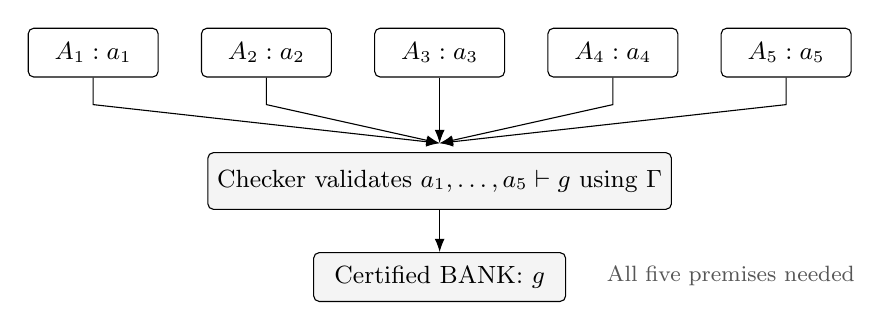
\begin{tikzpicture}[>=Latex,font=\small,host/.style={draw,rounded corners=2pt,minimum width=1.65cm,minimum height=.62cm,align=center},ctr/.style={draw,rounded corners=2pt,minimum width=4.5cm,minimum height=.72cm,align=center}]
\foreach \i/\x in {1/0,2/2.2,3/4.4,4/6.6,5/8.8} {
 \node[host] (h\i) at (\x,1.8) {$A_{\i}:a_{\i}$};
 \draw[->] (h\i.south) -- (\x,1.14) -- (4.4,.65);
}
\node[ctr,fill=papergray] (v) at (4.4,.17) {Checker validates $a_1,\ldots,a_5\vdash g$ using $\Gamma$};
\node[host,fill=papergray,minimum width=3.2cm] (g) at (4.4,-1.05) {Certified BANK: $g$};
\draw[->] (v) -- (g);
\node[anchor=west,text=mute,font=\footnotesize] at (6.4,-1.04) {All five premises needed};
\end{tikzpicture}
\caption{The five-way Horn witness. This is a logical dependence on evidence distribution. It does not imply that a central solver given the entire premise union is unable to prove $g$.}
\label{fig:horn}
\end{figure}

\section{The phrase ``under the same resource limits''}
\subsection{Three comparisons that must not be conflated}
The central question becomes ambiguous unless one specifies who possesses what and what counts as a resource. Consider the following comparisons:
\begin{center}
\small
\begin{tabularx}{\textwidth}{@{}p{.24\textwidth}X X@{}}
\toprule
\textbf{Comparison} & \textbf{What is held fixed?} & \textbf{What the Gestalt witness shows} \\
\midrule
Individual-view & Each ATP uses its own permitted $E_i$ and local computational allowance. & No individual derives $g$; federation with pooled authorized evidence does. \\
Equal aggregate effort & Federation total charged work is compared with one solver at the same budget, and both see the same initially available evidence. & No speedup follows merely from the witness. \\
Equal wall time & A concurrent federation and a sequential solver have a fixed elapsed-time horizon. & Parallel or specialized execution can help under a specified hardware model, but not automatically. \\
\bottomrule
\end{tabularx}
\end{center}
The first comparison proves a \emph{distributed-information separation}. It remains true even with unbounded individual search, as long as the missing premises are genuinely inaccessible. It is not an equal-information complexity lower bound. Giving a single ATP $\Sigma_0$ makes the Horn proof easy.

\subsection{A conditional no-free-speedup theorem}
\begin{theorem}[Cost-dominating simulation bound]\label{thm:sim}
Let $H_F$ be the successful cooperative histories for a frozen target and $H_B$ successful histories of a specified single-ATP baseline with the same permitted evidence. Let $C_F,C_B\ge0$ be declared total costs. If there is a map $T:H_F\to H_B$ such that
\[
C_B(T(\rho))\le C_F(\rho)\qquad\text{for all }\rho\in H_F,
\]
then, whenever $H_F\ne\varnothing$,
\[
\inf_{h\in H_B}C_B(h)\ \le\ \inf_{\rho\in H_F}C_F(\rho).
\]
\end{theorem}
\begin{proof}
For each $\rho\in H_F$, $\inf_{h\in H_B}C_B(h)\le C_B(T(\rho))\le C_F(\rho)$. Taking the infimum over $\rho$ proves the assertion.
\end{proof}

This is the same abstract bound as Theorem 10.1 of \cite{tenneson-dreaming}; it is restated to expose its assumptions. It proves \emph{no automatic gain when cost-dominating simulation exists}, not a theorem that a particular centralized program always satisfies the premise. A sequential interpreter can reproduce a completely logged finite distributed computation when all required state and external responses are available, typically with some serialization overhead; such replay need not match real-time parallel speed or multi-principal security properties. The scope-qualified finite-trace serialization argument is also discussed in \cite{tenneson-wcf}.

\begin{proposition}[No universal strict advantage over a baseline class containing the same method]
Fix a cost metric and a baseline class containing a single-ATP implementation that exactly simulates a proposed symphony-guided strategy at no greater cost. Under that metric and class, the symphony-guided strategy cannot have strictly lower cost than \emph{every} admissible baseline.
\end{proposition}
\begin{proof}
The simulating implementation is a member of the baseline class and is at most as costly. The required strict inequality fails for that member.
\end{proof}

\subsection{Full cost, rather than a count of proof lines}
For a finite run $\rho$, define the vector
\begin{equation}\label{eq:ledger}
\mathbf C(\rho)=(c_{\mathrm{search}},c_{\mathrm{check}},c_{\mathrm{storage}},c_{\mathrm{message}},c_{\mathrm{schedule}},c_{\mathrm{restart}},c_{\mathrm{recheck}},c_{\mathrm{score}}).
\end{equation}
The final coordinate accounts for musical encoding, indexing, decoding and any model training. For a publicly fixed weight vector $\mathbf w\ge0$, put $C_{\mathbf w}(\rho)=\mathbf w\cdot\mathbf C(\rho)$. The \emph{same-resource} claim must state whether it means equality of weighted total work, componentwise budget limits, hardware count, or a common wall-time deadline.

\begin{proposition}[A break-even condition for reusable motifs]
Suppose learning, encoding, storing, and validating a dream motif costs $k\ge0$ units once. Each of $m$ later uses saves $s\ge0$ search units while incurring $r\ge0$ extra retrieval, transport, and checking units. Against a baseline that repeats the original search, the score method gives strict total savings exactly when
\[
\boxed{m(s-r)>k.}
\]
\end{proposition}
\begin{proof}
Subtract the score method's incremental costs from the baseline's search costs. Net savings are $m(s-r)-k$, which are strictly positive precisely under the displayed inequality.
\end{proof}

\begin{example}[Symbolic, not empirical]
Let $k=20$, $s=8$, and $r=3$. Four reuses exactly break even; five yield a net advantage of five units. If verifier or message costs raise $r$ to $9$, no number of reuses provides savings under this model. This example is an accounting identity, not an ATP benchmark.
\end{example}

\section{What symphonies contribute to proof theory}
The term \emph{proof theory} has a narrow logical meaning---derivations, admissible rules, normalization, and the relationship of proof systems to their semantics---and a broader computational meaning involving representations and search for proof objects. SYMPHONY primarily belongs to the second domain unless it is equipped with new formally specified proof transformations.

\subsection{Theories and theorems are not created by music}
The underlying theory is $\Sigma_0$ together with a formal calculus. Its theorem set $\Cn(\Sigma_0)$ is invariant under certified, assumption-preserving changes of search representation. By \cref{thm:sound}, replacing a derivation heuristic with a symphony changes the \emph{route} to a certificate, not the set of valid conclusions. This reflects the invariant-core distinction in \cite{tenneson-core}.

\subsection{A symphony can index proof-relevant relationships}
The score, when adequately tagged, may preserve cross-member dependency graphs, repeated proof-subgoal motifs, temporal patterns of failed and successful lemma imports, or a provenance chain leading to a certificate. These are all mathematically expressible graph or trace properties. A retrieved motif can suggest the next search action, but the suggested formula or derivation remains a candidate until the checker accepts it. A sound but lossy index can still be useful if the full evidentiary packet is available separately.

\subsection{Potential meaning of harmony and counterpoint}
The musical metaphors can be made precise without mistaking metaphor for theorem. A \emph{voice} is a local event projection $\pi_i(\rho)$; a \emph{motif} is a recognizable, typed finite subtrace; \emph{counterpoint} is compatible interleaving of distinct voices; \emph{harmony} may be defined as a set of jointly satisfiable subgoal dependencies; and a \emph{cadence} may be defined as a verified terminal certificate. These are \emph{optional definitions}, not claims that tonal harmony logically entails theoremhood. Another theory could choose different musical interpretations while leaving the soundness proof unchanged.

\begin{table}[htbp]
\centering\small
\begin{tabularx}{\textwidth}{@{}p{.23\textwidth}p{.30\textwidth}X@{}}
\toprule
\textbf{Musical name} & \textbf{Mathematical candidate} & \textbf{Verification obligation}\\
\midrule
Voice & Ordered host projection & Correct provenance and event scope\\
Motif & Typed recurrent subtrace or proof pattern & Match is sound for the intended use\\
Counterpoint & Legally interleaved local events & Admissible ordering, no invalid imports\\
Harmony & Compatible subgoal/evidence constraints & Satisfiability or dependency checks\\
Cadence & Accepted terminal proof packet & Full independent proof-checker verdict\\
\bottomrule
\end{tabularx}
\caption{A proposed semantics for selected musical terms. The rightmost column prevents aesthetic descriptions from becoming unauthorized inference rules.}
\end{table}

\section{Limits, negative examples, and research obligations}
\subsection{Not every possible collection is a performance}
For a well-typed comparison, let $\operatorname{Dreams}_i(\rho)$ be the set of report-union dreams in host $i$'s projection of a global run. Define the global-run-induced local universe and the jointly realizable profile family by
\[
\Dream_i^{\mathcal F}(c)\defeq
 \bigcup_{\rho\in\Runs(\mathcal F,c)}\operatorname{Dreams}_i(\rho),\qquad
 \operatorname{Prof}(\mathcal F,c)\defeq
 \bigl\{(\operatorname{Dreams}_i(\rho))_{i=1}^{5}:\rho\in\Runs(\mathcal F,c)\bigr\}.
\]
Then
\[
\operatorname{Prof}(\mathcal F,c)\ \subseteq\
\prod_{i=1}^{5}\PSet\bigl(\Dream_i^{\mathcal F}(c)\bigr),
\]
with strict inclusion possible. For example, a single nonrenewable authorization token could be consumed by an $A_1$ dream or by an $A_2$ dream, each in a different legal run, but not by both in the same run. The Cartesian product contains the profile demanding both dreams; $\operatorname{Prof}(\mathcal F,c)$ does not. This comparison uses consistently typed tuples of dream sets. The richer $\Sym(\mathcal F,c)$ additionally carries ordered events, evidence provenance, and checker records; it is not itself a Cartesian product of local MUSIC families.

\subsection{No information can emerge from identical observable worlds}
If two possible external worlds induce the same authorized checkpoint, legal transition relation, readable evidence, and randomness distribution, a federation relying solely on that interface cannot reliably distinguish them, even if randomized. Coupling the same random choices yields identical observed traces by induction over legal transitions, so the output distributions also coincide. Accordingly, five dreamers do not obtain a fact that is absent from \emph{all} their admissible evidence merely through composition. The related indistinguishability claim appears as Proposition 11.1 in \cite{tenneson-dreaming}.

\subsection{No performance claim follows from an existence theorem}
The five-member construction establishes that some coordinated execution is possible and some proper coalitions lack the required premises. It does not show that the procedure is optimal, that a physical system has been installed, that a musical encoding improves recall, or that verified theorems are discovered at lower fully accountable cost. A rigorous experiment should use equal access to the relevant initial evidence when claiming \emph{algorithmic} advantage and should retain the restricted-access comparison separately when measuring \emph{distributed-information} advantage.

\subsection{A falsifiable symphony-advantage question}
\begin{question}[Certified symphony advantage]
For a specified class of proof problems, a declared resource vector, a documented certificate-faithful score design, and a preregistered set of strong equal-access baseline ATPs, can a five-member symphony-guided system achieve a statistically robust improvement in certified settlements per unit of fully accountable cost without increasing false acceptance?
\end{question}

This is deliberately an empirical research question. It cannot be decided by the Horn witness alone. Useful ablations include: (a) no federation exchange; (b) exchange without musical indexing; (c) musical indexing without cross-member exchange; (d) both exchange and indexing. These comparisons isolate whether any improvement comes from evidence pooling, search guidance, representation, or parallel hardware.

\section{A complete small worked trace}
A reader can reconstruct the core theorem without access to any other publication. Let the common formula be $(a_1\land\cdots\land a_5)\to g$, and suppose each member initially has a frozen authenticated packet for its $a_i$.
\begin{enumerate}[label=\textbf{Step \arabic*.},leftmargin=*]
\item \textbf{Local dreams.} Knowledge at $A_i$ reads its local packet; Awareness validates origin and time. Each member emits typed location reports whose union constitutes a dream. After authorized transmission, $A_1$ also dreams with a received $A_2$ packet, satisfying the cross-member condition.
\item \textbf{Proposals.} The Board records the tentative target $g$ and the list of five premises. Nothing has yet been deposited as a theorem.
\item \textbf{Score.} A structured musical representation records the five voice projections and the schedule, authenticated send/receive events, and evidence identifiers. The score is not an inference rule.
\item \textbf{Transport.} Player Zero authorizes receipt of each $a_i$ at $A_1$ or its approved shared interface. The recipient checks context, sender, and eligibility before using the packet; the post-receipt dream in Step 1 is ordered after its corresponding receipt.
\item \textbf{Proof object.} The proof-producing routine cites lines $a_1,\ldots,a_5$ as scoped premises, derives $a_1\land\cdots\land a_5$ by conjunction introduction, cites the Horn rule from $\Gamma$, and derives $g$ by implication elimination. The separate checker validates each proof step and its context.
\item \textbf{Acceptance.} The shared BANK adds $g$ under the original $\Sigma_0$ context. The acceptance-bearing event-prefix score is a certified movement because the chosen replay-faithful encoding permits reconstruction and independent rechecking of the full derivation.
\item \textbf{Counterfactual audit.} Remove any host $A_j$ and its evidence. The valuation $a_j=\mathrm{false}$, $g=\mathrm{false}$ witnesses that the remaining premises do not entail $g$.
\end{enumerate}
The example displays both the positive and negative obligations: joint proof construction and proper-coalition nonderivability. It is a mathematical model trace, not a log from an authenticated five-machine execution.

\section{Claim ledger and AMLD+0 settlement discipline}
\paragraph{Five investigative functions.} In an AMLD+0-\emph{style} reading of this paper, $P$ supplies \cref{thm:gestalt,thm:realize,thm:sound}; $R$ supplies the unordered-history and universal-speedup counterexamples; $D$ identifies access, proof scope, and cost dependencies; $I$ reports no certified independence statement; and $C$ audits inconsistent assumptions or unauthorized evidence imports. None of these labels denotes independently executed computational agents in this manuscript.

\paragraph{Settlement.} \textbf{P, for the restricted existential conjecture:} there is a legal, verifier-gated cooperative symphony that yields a certified proof unavailable to any individual restricted-evidence member. \textbf{R, for universal strict dominance against a baseline class that includes a cost-dominating simulator:} the stated universal advantage is refuted under that explicit premise. \textbf{U, for unspecified or empirical performance improvements:} the article contains no comparative benchmark establishing a gain under fully matched evidence and resource constraints. The proof's status is \emph{internally mathematically reviewed}, not externally machine certified.

\noindent\textbf{Evidence and claim classification.} The following ledger summarizes what is formalized in this manuscript and which claims remain conditional.
\begin{center}\small
\begin{tabularx}{\textwidth}{@{}>{\raggedright\arraybackslash}p{.29\textwidth}>{\raggedright\arraybackslash}p{.22\textwidth}>{\raggedright\arraybackslash}X@{}}
\toprule
\textbf{Claim} & \textbf{Status} & \textbf{Justification or limitation}\\
\midrule
Set-theoretic MUSIC exists & Proved given set-sized dream space & Definition and powerset recovery\\
A replay-faithful symphony score can exist & Constructive existence & Event-wise injective encoding with deterministic inverse\\
Five-member coalition-minimal proof & Proved & Horn witness and countervaluation; earlier source Theorem 6.2\\
Five-member legal dream run can certify target & Conditional existence & Explicit construction; earlier source Theorem 7.1 has stronger features\\
Verifier-gated global soundness & Conditional theorem & Induction on accepted deposits\\
Every symphony improves a real ATP & Not established & No benchmark or universal speedup theorem\\
Strictly beats every admissible equal-access baseline & Refuted if a cost-dominating simulator is included & Conditional simulation bound\\
\bottomrule
\end{tabularx}
\end{center}

\section{Conclusion}
A proof-producing ATP symphony is possible in a precise but conditional sense. Five hosts may jointly possess premises that no proper coalition possesses; a legal cooperative dreaming run can deliver those premises to a checker; and a replay-faithful, prefix-compatible score can encode the run without introducing an unsound inference. The decisive mathematical lesson is that \emph{jointly available evidence} is different from \emph{locally available evidence}, while \emph{evidence-preserving representation} is different from \emph{proof authority}. MUSIC names possible-dream families, while SYMPHONY names legal, temporally structured score realizations; only a specified certified-performance subfamily contains an accepted target proof. The additional claim that musical encoding yields superior proof-search economics is a separate, testable hypothesis.

\section*{Attribution and related work}
\addcontentsline{toc}{section}{Attribution and related work}
The original research architecture, the five-ATP dreaming model, the coalition-minimal Gestalt witness, the formal role distinctions, and the no-free-speedup framework are attributable to Brian Tenneson's referenced manuscripts. The proofs of source-derived results are reproduced so this article can stand on its own. The present symphony formulation makes explicit a structured score, joint legal realizability, certificate faithfulness, and the proof-theoretic versus empirical distinction. The mere terms MUSIC and SYMPHONY, or standard cardinality and factorization facts, do not independently establish novelty or academic priority. The \emph{MUSIC of an Automated Theorem Prover} companion article \cite{tenneson-music} treats the local powerset and realizability-complex foundations in greater detail; it is not needed to follow this article.

\begingroup\footnotesize

\section*{Notation and terminology}
\addcontentsline{toc}{section}{Notation and terminology}
\begin{tabularx}{\textwidth}{@{}p{.23\textwidth}X@{}}
$A_i$ & The $i$th ATP host, not the $i$th internal dream player.\\
$P_{i,k}$ & An internal player/process within host $A_i$.\\
$\Gamma, E_i,\Sigma_0$ & Shared background, member evidence, and frozen global premise union.\\
$\Cn(X)$ & Deductive closure of premises $X$ in the declared calculus.\\
$\Bank/\Board$ & Verified records versus provisional working hypotheses.\\
$\Dream_i(c_i)$ & Possible report-union dreams at a frozen local condition.\\
$\Music_i$ & Powerset of all locally possible dreams.\\
$K_i$ & Finite jointly realizable collections of local dreams.\\
$\pi_i(\rho)$ & Host $i$'s ordered projection of a legal federation run.\\
$H_\rho,Q_\rho,G_\rho$ & Causal order, authenticated verification ledger, and global/control event ledger.\\
$S(\rho)$ & Structured musical score of a legal run.\\
$\Sym(\mathcal F,c)$ & All legal scores from checkpoint $c$, whether or not they certify a target.\\
$\Sym_g^{\mathrm{cert}}$ & Scores with a witnessing run that accepts a checked proof for $g$.\\
$\operatorname{Prof}(\mathcal F,c)$ & Tuples of jointly realized local dream sets in one global execution.\\
$V$ & Independent checker under the frozen proof contract.\\
\end{tabularx}

\begin{thebibliography}{9}
\setlength{\itemsep}{0pt}\setlength{\parsep}{0pt}
\bibitem{tenneson-dreaming}
B. Tenneson, \emph{Dreaming in a Five-ATP Federation: One AMLD+0 Conjecture Settler, Five ATP Members, Certified Dreaming, and Self-Directed Mathematical Study}, Research Manuscript 0.4R (ATLAS-repaired), October 29, 2026. Especially Definition 6.1; Theorems 4.1, 4.2, 6.2, 7.1, 10.1; and Propositions 11.1--11.2.\newline
\footnotesize\url{https://btenneson.github.io/pub/cs.LO_Logic_in_Computer_Science/five_atp_one_amld_dreaming_0_4r_atlas_repaired/}\normalsize

\bibitem{tenneson-core}
B. Tenneson, \emph{The Invariant Core and the Geometry of Settlement}, research article, 2026.\newline
\footnotesize\url{https://btenneson.github.io/pub/cs.LO_Logic_in_Computer_Science/invariant_core_geometry_settlement/}\normalsize

\bibitem{tenneson-wcf}
B. Tenneson, \emph{Who Checks the Federation? Non-Singleton Settlement, Certified Cooperation, and the AMLD+0 Research Program}, Integrated Research Edition 7.10, November 3, 2026. Especially the formal federation architecture, conservative certified growth, finite trace serialization, and full cost ledger.\newline
\footnotesize\url{https://drive.google.com/file/d/14ud5bXYnV5dfWGsFjF9Byq2uKy--lA-r/view}\normalsize

\bibitem{tenneson-bootstrap}
B. Tenneson, \emph{AMLD+0 --- Conversational Operations Bootstrap}, \texttt{AMLD0\_ChatGPT\_Bootstrap\_REGEN.md}, November 3, 2026. A proposed structured conversational protocol, not evidence of a separately deployed five-agent federation.\newline
\footnotesize\url{https://drive.google.com/file/d/1CQ5Wo-TUMYcIXtmehPUFZ6zd56bDuCjQ/view}\normalsize

\bibitem{tenneson-music}
B. Tenneson, \emph{MUSIC of an Automated Theorem Prover: Possible Dream Families, Realizability Complexes, and Certified Reflection}, version 2.0, companion AI-assisted research exposition, November 3, 2026.\newline
\footnotesize\url{https://btenneson.github.io/pub/cs.LO_Logic_in_Computer_Science/music_of_an_atp_expository_research_article_2_0/}\normalsize

\bibitem{lamport}
L. Lamport, ``Time, Clocks, and the Ordering of Events in a Distributed System,'' \emph{Communications of the ACM}, 21(7), pp. 558--565, 1978, doi:10.1145/359545.359563. Relevant to causal ordering of distributed event records; not a source for the MUSIC definition.

\bibitem{herlihy}
M. Herlihy, D. Kozlov, and S. Rajsbaum, \emph{Distributed Computing Through Combinatorial Topology}, Morgan Kaufmann/Elsevier, first edition released November 2013 (copyright 2014). General context for complexes of compatible distributed states; not a direct antecedent of the named ATP symphony.
\end{thebibliography}
\endgroup

\clearpage
\thispagestyle{plain}
\vspace*{10mm}
\begin{center}
{\Large\bfseries AI Authorship and Mathematical Reliability Disclaimer}\par
\vspace{3pt}{\small Full statement on the final page}
\end{center}
\vspace{9pt}
This manuscript is a human-originated, AI-assisted research exposition. Brian Tenneson supplied the research program, earlier source theorems, the concept of ATP dreaming on generalized board games, the definition of MUSIC as the set of sets of possible dreams conditional on BANK/players/initial or intermediate conditions, and the proposed application to a federation ``symphony.'' ChatGPT (GPT-6) assisted with formal notation, reconstruction of the source arguments, mathematical exposition, counterexamples, new proposed definitions, diagrams, bibliography, and document preparation. The present Atlas audit denotes iterative manuscript review and repair, not an independent formal checker or authenticated multi-agent execution. Other names or prior editorial audits in the source works do not attest that those systems independently verified this article.

\medskip
Every effort has been made to present relevant facts, conditions, mathematical arguments, definitions, and limits in a factually accurate, logically coherent, and useful exposition. ``Complete'' in this editorial context means covering relevant assumptions and information, not technical completeness in formal logic. The paper offers no guarantee that every statement is correct, consistent, formally provable, novel, free of overlooked hypotheses, or resistant to counterexample or future correction. The mathematical proofs presented here have been reviewed in the course of AI-assisted drafting but have not been checked by an independent formal proof assistant or authenticated automated federation. The examples are constructed models, not logs of actual five-host executions; conditional theorems are not empirical performance measurements.

\medskip
No dream, musical score, symphony, role narrative, or chat-generated proof sketch is by itself an external proof certificate. The distinction between Board exploration and independently checked BANK admission is essential. Readers should verify the cited antecedent results and the new derivations, assess exact resource and evidence assumptions before comparing systems, and avoid interpreting an existence theorem as proof of a deployed, faster, or globally original implementation.

\vfill
\begin{center}\small\itshape End of manuscript\end{center}
\end{document}